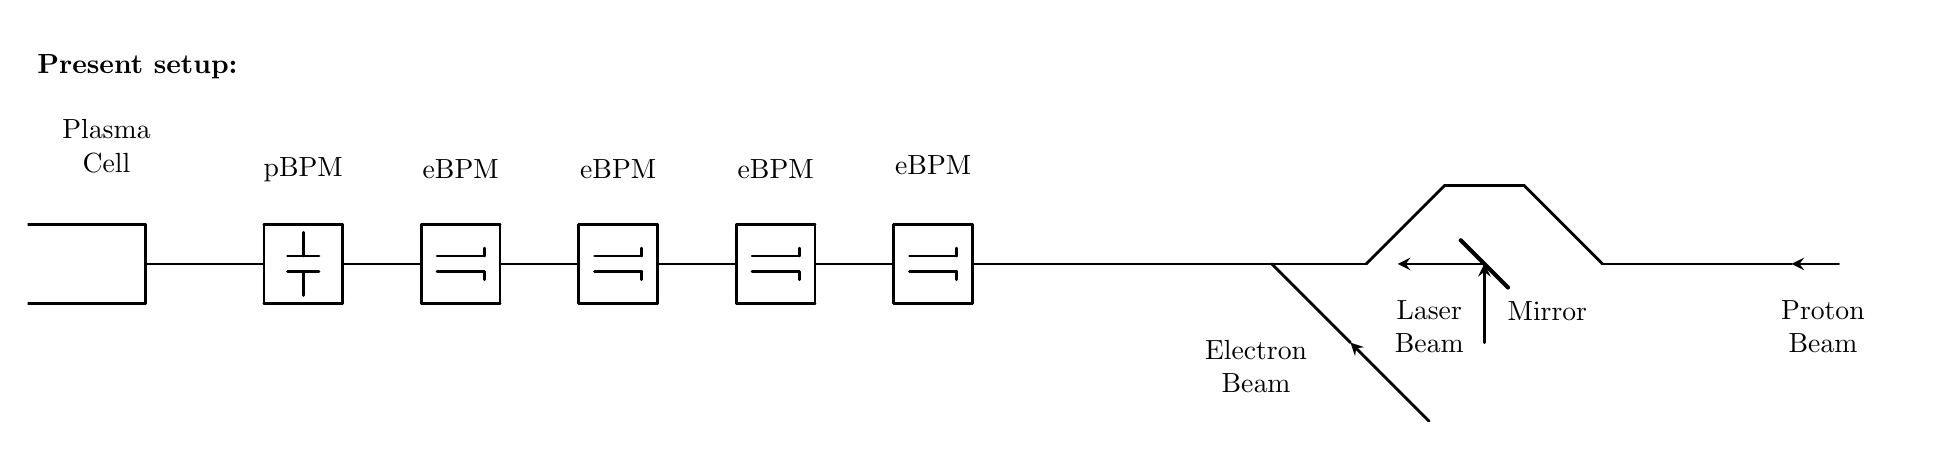
\begin{tikzpicture}[line cap=round,line join=round,>=stealth,x=1cm,y=1cm]
% new version
\clip(-10,-2) rectangle (14, 3);
\draw (-10.,2.5) node[anchor=west] {\textbf{Present setup:}};
\draw [line width=1pt] (-10,0.5)-- (-8.5,0.5);
\draw [line width=1pt] (-8.5,0.5)-- (-8.5,-0.5);
\draw [line width=1pt] (-8.5,-0.5)-- (-10,-0.5);
\draw (-9.,1.5) node[anchor=center] {\parbox{4cm}{\centering Plasma\\Cell}};
\draw [line width=1pt] (-7,0.5)-- (-7,-0.5);
\draw [line width=1pt] (-6,-0.5)-- (-6,0.5);
\draw [line width=1pt] (-6,0.5)-- (-7,0.5);
\draw [line width=1pt] (-7,-0.5)-- (-6,-0.5);
\draw [line width=1pt] (-5,0.5)-- (-5,-0.5);
\draw [line width=1pt] (-5,-0.5)-- (-4,-0.5);
\draw [line width=1pt] (-4,-0.5)-- (-4,0.5);
\draw [line width=1pt] (-4,0.5)-- (-5,0.5);
\draw [line width=1pt] (-3,0.5)-- (-3,-0.5);
\draw [line width=1pt] (-3,-0.5)-- (-2,-0.5);
\draw [line width=1pt] (-2,-0.5)-- (-2,0.5);
\draw [line width=1pt] (-2,0.5)-- (-3,0.5);
\draw [line width=1pt] (-1,0.5)-- (0,0.5);
\draw [line width=1pt] (0,0.5)-- (0,-0.5);
\draw [line width=1pt] (0,-0.5)-- (-1,-0.5);
\draw [line width=1pt] (-1,-0.5)-- (-1,0.5);
\draw [line width=1pt] (1,0.5)-- (1,-0.5);
\draw [line width=1pt] (1,-0.5)-- (2,-0.5);
\draw [line width=1pt] (2,-0.5)-- (2,0.5);
\draw [line width=1pt] (2,0.5)-- (1,0.5);
\draw [line width=1pt] (6,0)-- (5,0);
\draw [line width=1pt] (6,0)-- (7,0);
\draw [line width=1pt] (7,0)-- (8,1);
\draw [line width=1pt] (8,1)-- (9,1);
\draw [line width=1pt] (9,1)-- (10,0);
\draw [line width=1pt] (10,0)-- (11,0);
\draw [line width=1pt] (-8.5,0)-- (-7,0);
\draw [line width=1pt] (-6,0)-- (-5,0);
\draw [line width=1pt] (-4,0)-- (-3,0);
\draw [line width=1pt] (-2,0)-- (-1,0);
\draw [line width=1pt] (0,0)-- (1,0);
\draw [line width=1pt] (2,0)-- (5,0);
\draw [line width=1pt] (-2.8,0.1)-- (-2.2,0.1);
\draw [line width=1pt] (-2.2,0.1)-- (-2.2,0.2);
\draw [line width=1pt] (-2.8,-0.1)-- (-2.2,-0.1);
\draw [line width=1pt] (-2.2,-0.1)-- (-2.2,-0.2);
\draw [line width=1pt] (-0.8,0.1)-- (-0.2,0.1);
\draw [line width=1pt] (-0.2,0.1)-- (-0.2,0.2);
\draw [line width=1pt] (-0.8,-0.1)-- (-0.2,-0.1);
\draw [line width=1pt] (-0.2,-0.1)-- (-0.2,-0.2);
\draw [line width=1pt] (1.2,0.1)-- (1.8,0.1);
\draw [line width=1pt] (1.8,0.1)-- (1.8,0.2);
\draw [line width=1pt] (1.2,-0.1)-- (1.8,-0.1);
\draw [line width=1pt] (1.8,-0.1)-- (1.8,-0.2);
\draw [line width=1pt] (-4.8,0.1)-- (-4.2,0.1);
\draw [line width=1pt] (-4.2,0.1)-- (-4.2,0.2);
\draw [line width=1pt] (-4.8,-0.1)-- (-4.2,-0.1);
\draw [line width=1pt] (-4.2,-0.1)-- (-4.2,-0.2);

\draw [line width=1pt] (-6.7,-0.1)-- (-6.3,-0.1);
\draw [line width=1pt] (-6.7,0.1)-- (-6.3,0.1);
\draw [line width=1pt] (-6.5,0.1)-- (-6.5,0.4);
\draw [line width=1pt] (-6.5,-0.1)-- (-6.5,-0.4);

\draw (-6.5,1.2) node[anchor=center]  {pBPM};;
\draw (-4.5,1.2) node[anchor=center] {eBPM};
\draw (-2.5,1.2) node[anchor=center] {eBPM};
\draw (-0.5,1.2) node[anchor=center] {eBPM};
\draw (1.5,1.25) node[anchor=center] {eBPM};
\draw [line width=1.5pt] (8.2,0.3)-- (8.8,-0.3);
\draw [->,line width=1pt] (8.5,-1) -- (8.5,0);
\draw [->,line width=1pt] (8.5,0) -- (7.4,0);
\draw (7.8,-0.8) node[anchor=center]  {\parbox{4cm}{\centering Laser\\Beam}};;
\draw (9.3,-0.6) node[anchor=center] {Mirror};
\draw [->,line width=1pt] (13,0) -- (12.4,0);
\draw [line width=1pt] (12.4,0)-- (11,0);
\draw (12.8,-0.8) node[anchor=center]  {\parbox{4cm}{\centering Proton\\Beam}};;
\draw [line width=1pt] (5.8,0)-- (6.8,-1);
\draw [->,line width=1pt] (7.8,-2) -- (6.8,-1);
\draw (5.6,-1.3) node[anchor=center]  {\parbox{4cm}{\centering Electron\\Beam}};;


\end{tikzpicture}
